


\chapter{Estado del Arte}\label{chapter:state-of-the-art}
En este capítulo se brindan las definiciones de herramientas utilizadas para la autenticacióna. También se realiza un estudio sobre el estado del arte de las mismas. Además, se brindan razones para incluir su utilización como parte de la solución propuesta.\\
\textcolor{blue}{Si quieres en lugar de este pequeño parrafo introductorio haz un resumen de todo lo que hablas en el capítulo }

\textcolor{blue}{Recuerda que tu estado del arte va sobre autenticación. \\
	Puedes salirte un poco de autenticación central y hablar de otras formas de autenticar ( radius, kerberos, active directory u otros protocolos que te encuentres )}\\\\


\section{Inicio de Sesión Único}
\textcolor{blue}{Tienes una perfecta definición en el párrafo a continuación. Pero como que queda un poco seca no crees ? Quien lo usa, desde cuando se emplea. Que ventajas y desventajas posee. Ejemplos de softwares que lo usan. Son de código abierto ? Son de código cerrado ? \\
Por ahi tienes bastante tela por donde cortar. Lo mismo aplica para el resto de los protocolos de autenticación.}

El Inicio de Sesión Único ( en inglés \textit{Single Sign-On} o también conocido por sus siglas SSO) ha sido ampliamente adoptado para la autenticación en línea debido a su utilidad y seguridad que ofrece. Este es un método de autenticación que permite a los usuarios iniciar sesión con un único conjunto de credenciales en varios sistemas de software independientes. El inicio de sesión único facilita que un usuario no tenga que iniciar sesión en cada aplicación que use. Con este servicio los usuarios pueden acceder a todas las aplicaciones necesarias sin tener que autenticarse con otras credenciales.[\cite{microsoft-doc}]

En el mundo digital actual, los usuarios acceden a múltiples sistemas para llevar a cabo sus quehaceres. A medida que aumenta la cantidad de sistemas, también aumenta la cantidad de credenciales de cada usuario y, por lo tanto, también incrementa la posibilidad de perderlas u olvidarlas. El inicio de sesión único se puede utilizar para resolver muchos problemas relacionados con múltiples credenciales para diferentes aplicaciones. El acceso de inicio de sesión único al centro de autenticación principal permite a los usuarios obtener acceso a todos los demás recursos disponibles. SSO ayuda a mejorar la productividad del usuario y del desarrollador al evitar que el usuario recuerde varias contraseñas y también reduce la cantidad de tiempo que el usuario dedica a escribir varias contraseñas para iniciar sesión. SSO también simplifica la administración mediante la gestión de credenciales únicas en lugar de múltiples credenciales. Facilita la gestión de los derechos de un usuario que llega, cambia de función dentro o sale de la empresa, para integrar rápidamente aplicaciones adicionales, delegar derechos de acceso durante las vacaciones sin aumentar la carga de trabajo de la mesa de ayuda. [\cite{radha2012survey}]

Grandes empresas como Google, Facebook y Microsoft utilizan estos servicios. En particular Google permite a sus usuarios iniciar sesión una única vez para tener acceso a todos los servicios de la empresa que se encuentran en la nube. Cuando se configura SSO, los usuarios pueden iniciar sesión en terceros proveedores de identidad y luego acceder a las aplicaciones de Google directamente sin un segundo inicio de sesión [\cite{google-support}]. Por ejemplo, si se accede a un servicio de Google como Gmail, se autentica automáticamente en YouTube, AdSense, Google Analytics, y otras applicaciones de Google. Del mismo modo, si cierra la sesión de su Gmail u otras aplicaciones de Google, se cerrará automáticamente la sesión de todas las aplicaciones; esto se conoce como Cierre de Sesión Único (en inglés: \textit{Single Logout}) [\cite{sso-doc}]

\subsection{Tipos de SSO}
The various types of SSO shown in Fig: 1, fall under different categories, based on where they are deployed (Intranet, Extranet, Internet); how they are deployed (architecture – Simple, Complex); the credentials they use (token, certificate..) and the protocols they use (Kerberos, SAML, OpenID..).Following picture shows the types of SSO and their classification: 

\begin{figure}[H]
	\centering
	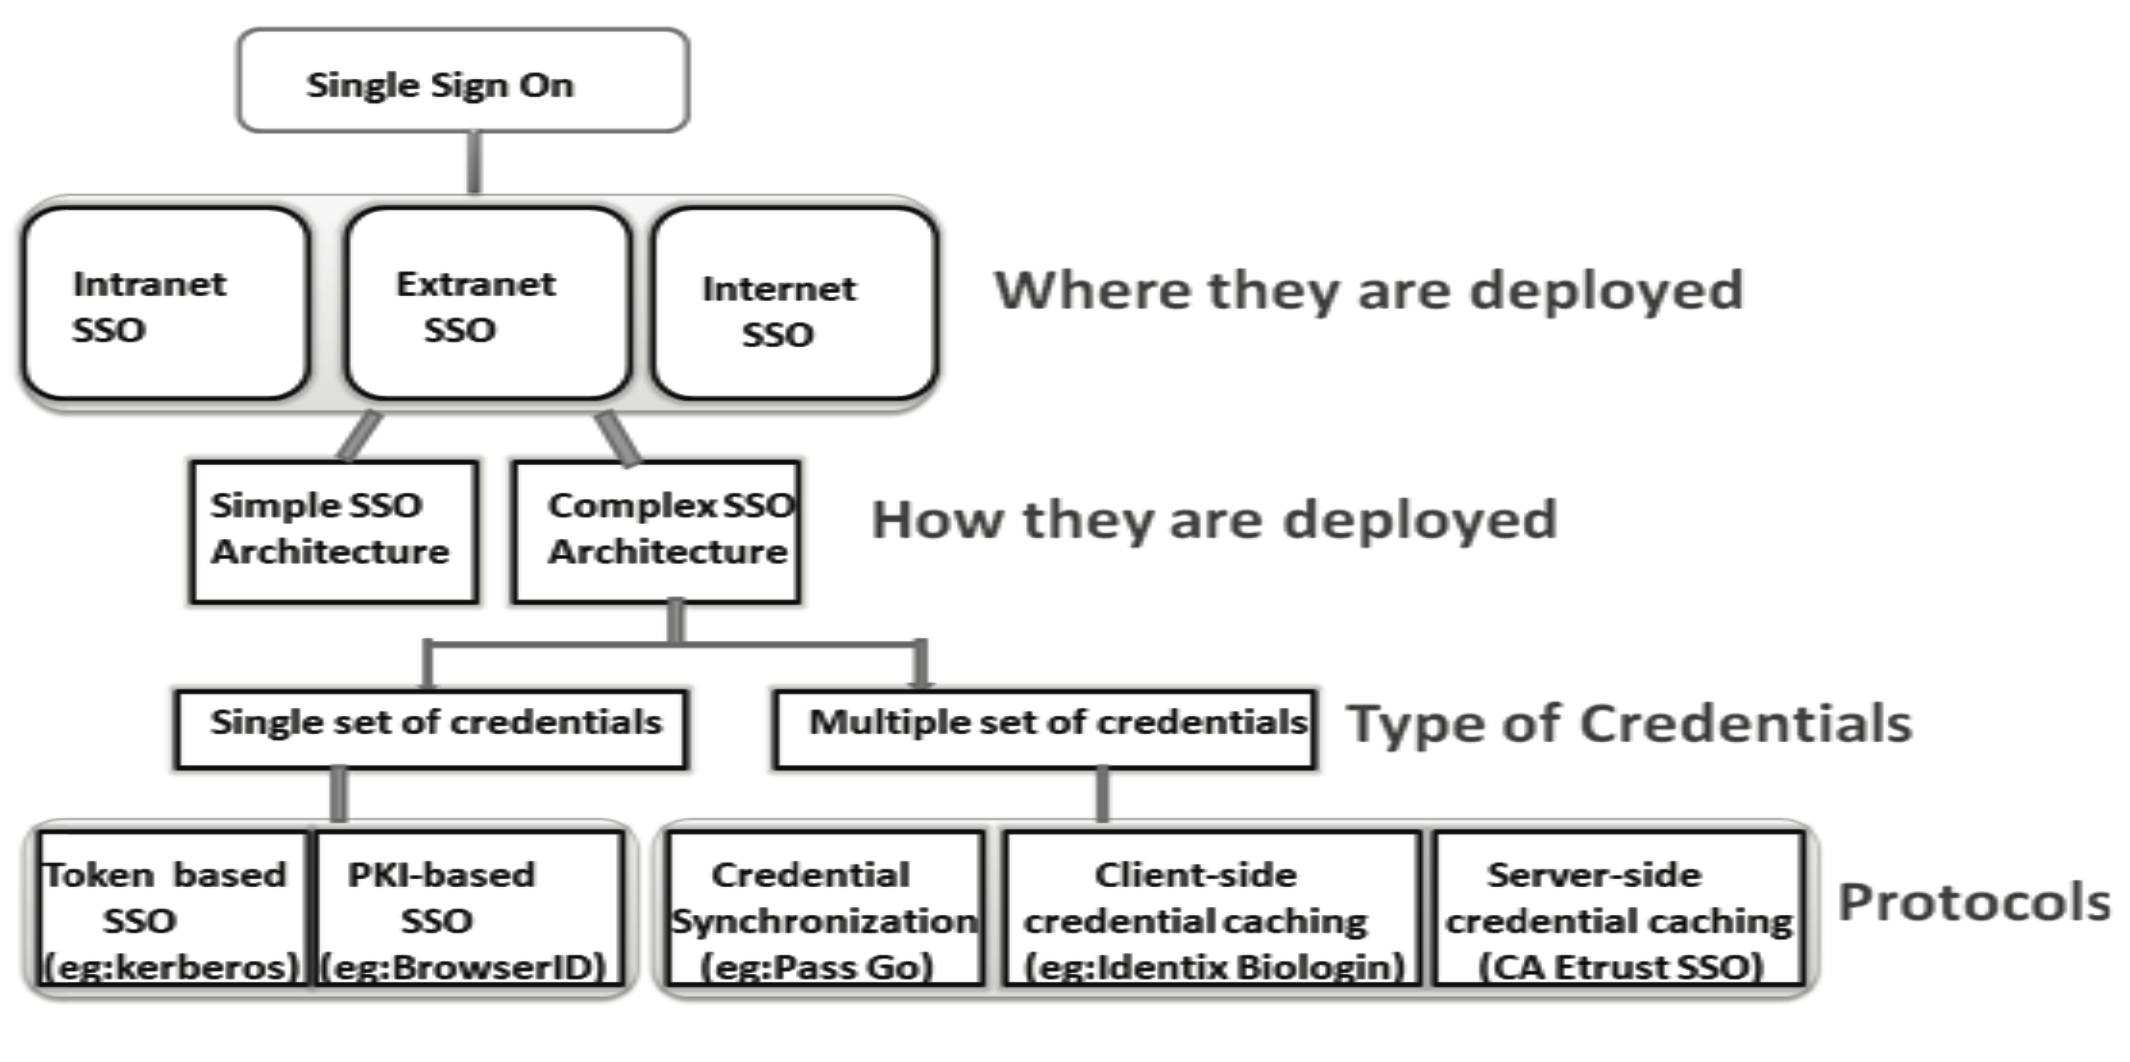
\includegraphics[width=0.7\linewidth]{Graphics/sso_types}
	\caption{}
	\label{fig:Tipos de SSO}
\end{figure}

Dadas las condiciones de la Universidad, se despliegará en Extranet ya que \textcolor{red}{Multi-domain SSO allows connecting to multiple systems within the same enterprise and all the business partners’ applications. The user can login into one enterprise and access resources of the other, the users need not login again using different credentials.}

Se despliegará con una arquitectura de tipo SSO compleja ya que \textcolor{red}{Complex SSO uses multiple authentication authorities with single or multiple sets of credentials for each user.}

En este caso se utilizarán un único conjunto de credenciales basado en tokens porque \textcolor{red}{In this SSO system, a user submits the credentials to the token-based authentication authority, in which the credentials have been checked with its credential database. If the user credentials match, then the user is returned with a token. When the user wants to access an application server which is governed by second authentication authority, the same token is delivered to get a ticket to access the application server. Success of this process relies on the trust the authentication authorities have among themselves.}

[\cite{radha2012survey}]

\section{OpenID Connect}
\textcolor{blue}{Hay una noción o distinción importante a la hora de diferenciar protocolos y que puedes abordar en tu estado del arte. Cada uno de los protocolos diseñados tiene como objetivo una arquitectura de red predeterminada. \\
Si bien OpenId Connect se diseño para entornos de internet donde no se puede verificar la autenticidad de los dispositivos clientes, también sirve para entornos mas controlados ( como puede ser la universidad )\\
Sin embargo, kerberos, radius y ldap si son pensados para redes controladas. ( privadas )}


\textit{OpenID Connect} es una capa de identidad simple implementada a partir del protocolo \textit{OAuth 2.0}. Permite a los clientes verificar la identidad del usuario final en función de la autenticación realizada por un servidor de autorización, así como obtener información básica del perfil del Usuario final de manera interoperable y similar al protocolo REST. [\cite{openid-doc}]. 

\textit{OpenID Connect }es uno de los protocolos de tipo \textit{Single Sign-On} más utilizados para delegar la autenticación. También tiene un formato simple, por lo que ha ganado popularidad y es soportado por grandes empresas como Google, IBM, Microsoft, Amazon y PayPal [\cite{mainka2017sok}]. La nueva versión es compatible con \textit{API} y puede ser usado por aplicaciones nativas y móviles. También define mecanismos opcionales más robustos para firmas y cifrados. [\cite{openid-doc}]

Este protocolo está basado en \textit{OAuth 2.0} por lo que tiene todas las ventajas de este protocolo. Sin embargo, lo extiende ya que ofrece facilidades para obtener más información de la identidad de los usuarios eficientemente. Permite un flujo de información adicional que genera un \textit{id-token} que contiene datos del usuario. De esta forma las aplicaciones no solo tienen acceso a los permisos de los usuarios, sino también obtienen información sobre la identidad de los usuarios.  [\cite{openid-doc}][\cite{kutera2016single}]

\section{SAML}
\textcolor{red}{ The Security Assertion Markup Language (SAML) defines the syntax and processing semantics of
assertions made about a subject by a system entity. In the course of making, or relying upon such
assertions, SAML system entities may use other protocols to communicate either regarding an assertion
itself, or the subject of an assertion. This specification defines both the structure of SAML assertions, and
an associated set of protocols, in addition to the processing rules involved in managing a SAML system. [\cite{philpott2015assertions}]
\\
SAML, developed by the Security Services Technical Committee of the Organization for the Advancement of Structured Information Standards (OASIS), is an XML-based framework for communicating user authentication, entitlement, and attribute information. As its name suggests, SAML allows business entities to make assertions regarding the identity, attributes, and entitlements of a subject (an entity that is often a human user) to other entities, such as a partner company or another enterprise application. SAML is a flexible and extensible protocol designed to be used – and customized if necessary
– by other standards. [\cite{wisniewski2005saml}]}

\section{LDAP}
El Protocolo Ligero de Acceso a Directorios (en inglés: \textit{Lightweight Directory Access Protocol}, también conocido por sus siglas de LDAP) es un conjunto de protocolos de licencia abierta que son utilizados para acceder a la información que está almacenada de forma centralizada en una red. Este protocolo se utiliza a nivel de aplicación para acceder a los servicios de directorio remoto. [\cite{ldap-doc}]

LDAP está basado en estándares implementados sobre TCP/IP \textcolor{blue}{Y Open Id Connect ?}. Permite a los clientes interactuar directamente con los servidores de los directorios: almacenar y consultar información, buscar datos filtrados, autenticar usuarios, entre otros.

Este protocolo es utilizado actualmente por muchos sistemas que apuestan por el software libre al utilizar distribuciones de Linux para ejercer las funciones propias de un directorio activo en el que se gestionarán las credenciales y permisos de los usuarios y estaciones de trabajo en redes LAN corporativas en conexiones cliente/servidor \textcolor{blue}{mientras que open id connect y el flujo de emisión de tokens esta pensado para redes abiertas ( internet )}.

Un directorio remoto es un conjunto de objetos que están organizados de forma jerárquica, tales como: nombre, claves, direcciones, etc. Estos objetos estarán disponibles para una serie de clientes conectados mediante una red, normalmente interna o LAN, y proporcionarán las identidades y permisos para esos usuarios que la utilicen.

\textcolor{blue}{Sería bueno que a cada protocolo le incluyas una url con el rfc que lo define ( cualquiera de ellos, el primero o el último ) ( puede haber mas de un rfc por protocolo )
\\
Ahora si esta en tu objetivo de tesis entender un protocolo, su link lo pones en la bibliografía consultada, por el contrario si es adicional, ponlo como un pie de página.}

LDAP está basado en el protocolo X.500 para compartir directorios, y contiene esta información de forma jerarquizada y mediante categorías para proporcionarnos una estructura intuitiva desde el punto de vista de la gestión por parte de los administradores.

Estos directorios se utilizan generalmente para contener información virtual de usuarios, para que otros usuarios accedan y dispongan de información acerca de los contactos que están aquí almacenados. Además es capaz de comunicarse de forma remota con otros directorios LDAP situados en servidores que pueden estar en el otro lado del mundo para acceder a la información disponible. De esta forma se crea una base de datos de información descentralizada y completamente accesible.
 
El sistema de autenticación vigente en el Nodo Central verifica sus usuarios con dos sistemas implementados con LDAP. Este protocolo se adapta a las necesidades y condiciones actuales de la Universidad ya que es \textit{Open Source} (OSS o código abierto).
\textcolor{red}{
	- It is a mature, flexible, and well supported standards-based mechanism for interacting with directory servers. It’s often used for authentication and storing information about users, groups, and applications, but an LDAP directory server is a fairly general-purpose data store and can be used in a wide variety of applications. \\ LDAP is a tool in the User Management and Authentication category of a tech stack.}


\section{Active Directory}


\section{Keycloak}
Keycloak es un software de código abierto que permite el \textit{Single Sign-On} o Inicio de Sesión Único con \textit{Identity Management} y \textit{Access Management} para aplicaciones y servicios modernos. Esta herramienta facilita la protección de aplicaciones y servicios con poca o ninguna codificación. Un Proveedor de identidad (en inglés: \textit{Identity Provider}, también conocido por sus siglas IdP), permite que una aplicación (a menudo llamada \textit{Service Provider} o SP) delegue su autenticación. [\cite{KeycloakDoc}]

Este software está escrito en Java y es compatible de forma predeterminada con los protocolos de federación de identidad SAML v2 y OpenID Connect (OIDC) / OAuth2. Está bajo licencia de Apache y es  mantenido por Red Hat. [\cite{KeycloakDoc}]

	\subsection{Características}
	Los usuarios se autentican en Keycloak en lugar de hacerlo en las aplicaciones. Esto significa que no es necesario que cada aplicación tenga un formulario de inicio de sesión, autentique a los usuarios o almacene sus datos. Una vez entren en Keycloak, los usuarios no tendrán que iniciar sesión en las demás aplicaciones conectadas al software.
	
	Lo mismo sucede cuando un usuario cierra sesión. Keycloak ofrece cierre de sesión único, lo cual significa que los usuarios solo tienen que desconectarse en una de las aplicaciones para salir de su cuenta en el resto. 
	
	Otra prestación de Keycloak son las federaciones de usuarios, que facilitan la compatibilidad con LDAP y otros servidores de directorios activos. También admite la implementación de servicios propios para usuarios guardados en otros tipos de almacenamientos como en bases de datos relacionales. 
	
	Keycloak ofrece como herramienta una consola de administración de cuentas, a través de la cual los usuarios pueden administrar sus propias cuentas. Pueden actualizar su perfil, cambiar sus contraseñas y configurar la autenticación en dos pasos. También pueden administrar sus sesiones y visualizar el historial de su cuenta. 
	
	Otra característica es que es una herramienta extensible porque permite la eliminación, adición y modificación de las bases de datos de usuarios, los métodos de autenticación y los protocolos. Está basada en protocolos estándares y soportan OpenID Connect, OAuth 2.0 y SAML. [\cite{KeycloakDoc}]
	
	Keycloak facilita añadir la autenticación y un servicio seguro a aplicaciones. Permite que los desarrolladores se centren en la funcionalidad empresarial al no tener que preocuparse por los aspectos de seguridad de la autenticación. También posibilita la unificación de los métodos de autenticación de distintas aplicaciones sin modificarlas.
	
%	\textcolor{red}{\textbf{Comparación}}
%	\textcolor{red}{Gluu: \\ Free open source access management suite with support for SAML and OpenID Connect SSO, and OAuth2 based web and API access management. The Gluu Server can include multiple components. Each one fulfills a different requirement, and can be included or excluded in individual deployments based on an organization’s unique requirements.}
%	\textcolor{red}{Gluu vs Keycloak: \\
%		- The Keycloak system requires 512 Mb of RAM and 1 GB of disk space, whereas the Gluu system requires 8 GB of RAM and 40 GB of disk space. \\ - Gluu is less flexible to extend} [\cite{vassallo2017continuous}]
	\textcolor{blue}{Que empresa usa KeyCloack, Que empresa usa Gluee ? Desde que año estan en el mercado?}\\
	\textcolor{red}{Gluu es otra de las tecnologías que tienen prestaciones y ventajas similares a Keycloak. Es un servicio \textit{Open Source} que soporta \textit{SMAL}, \textit{OpenID Connect, SSO} y \textit{OAuth 2.0}. Sin embargo Gluu es un sistema que requiere de 8 GB de RAM y 40 GB de espacio en disco, mientras que Keycloak solo necesita de 512 Mb de RAM y 1 GB de disco. Por ello Keycloak se ajusta más a los recursos que se tienen en la Universidad de La Habana.}
	
	
	\textcolor{blue}{Que otras soluciones de SSO existen en la industria ? ( Google, Facebook, Incluso Telegram permiten integración con SSO )}
	\\
	\textcolor{blue}{Otro punto a seguir puede ser que soluciones de autenticación se poseen para redes corporativas  (cerradas )\\
	poner ejemplos, hablar de ellas y etc ( keycloak y gluee sirven para eso también )}
	\\
	\textcolor{blue}{Y finalmente puedes hablar del estado de la autenticación de la Universidad de La Habana, puedo, si quireres por servicio, mencionarte el protocolo que se emplea para la autenticación}
	\\
	\textcolor{blue}{Recuerda, tu estado del arte va de autenticación. Hay mucha tela por donde cortar aca. No te limites a lo que hay en la uh. Todo lo que se autentique hoy en internet puede estar en tu tesis ( protocolo )}
	
	\textcolor{red}{
	\subsection{Google Authenticator}
	Millions of web users today use their Google accounts to sign into millions of relying party websites. This is enabled through the Google authentication API, which allows third party application developers to embed Google sign-in into their application. However, regardless to the strength of the Google authentication mechanism, the majority of these applications have been identified to be infected with broken authentication, which made them vulnerable to cyber attacks. A major reason for this is mistakes that developers make while embedding Google sign-in into their application. High complexity and lack of usability of the Google authentication API makes it difficult for programmers to use it correctly and lead them to make mistakes while using the API. [\cite{wijayarathna2019empirical}]
	\\
	We discussed how these usability issues would affect the security of the application that are developed using the Google authentication API and how the API should be improved to provide a better experience to application developers. [\cite{wijayarathna2019empirical}]}

\section{Seguridad}
\textcolor{red}{
Although security is a crucial aspect of any application, its implementation can be difficult. Worse, it is often neglected, poorly implemented and intrusive in the code. But lately, security servers have appeared which allow for outsourcing and delegating all the authentication and authorization aspects. Of these servers, one of the most promising is Keycloak, open-source, flexible, and agnostic of any technology, it is easily deployable/adaptable in its own infrastructure.}